\chapter{Frontend}

O \textit{frontend} da aplicação tem como principal objetivo fornecer uma 
interface intuitiva e interativa para que os utilizadores possam aceder às 
funcionalidades do clube, nomeadamente a adesão de sócios, a inscrição de 
atletas, o registo de patrocínios e a compra de bilhetes, bem como permitir a 
gestão destas áreas por parte dos utilizadores responsáveis.

Esta interface é construída como uma SPA (\textit{Single Page 
Application}), ou seja, uma aplicação de página única, na qual a 
navegação entre as diferentes secções não implica o recarregamento da página. 
Foi desenvolvida na linguagem TypeScript, uma linguagem 
fortemente tipificada que se baseia em JavaScript e que permite uma maior 
segurança em tempo de desenvolvimento e a deteção antecipada de erros. Para a 
construção da interface foi utilizada a biblioteca React~\cite{react}, que 
permite a construção de interfaces baseadas em componentes reutilizáveis, com 
atualização e renderização eficientes através de uma DOM virtual.

O empacotamento e o ambiente de desenvolvimento são geridos pela ferramenta 
Vite~\cite{vite}, que oferece um servidor de desenvolvimento rápido e um 
processo de \textit{build} otimizado. Durante o desenvolvimento, o Vite está 
ainda configurado para reencaminhar os pedidos dirigidos à API para o servidor 
do \textit{backend}, o que simplifica a comunicação entre as duas componentes.

No que diz respeito ao aspeto visual, a aplicação combina duas abordagens. Por 
um lado, recorre ao Tailwind CSS~\cite{tailwind}, uma \textit{framework} de CSS 
utilitária que define um tema próprio (paleta de cores, tipografia e animações) 
alinhado com a identidade visual do clube. Por outro, utiliza folhas de estilo 
de CSS próprias, organizadas por funcionalidade, para os estilos mais 
específicos de cada área da aplicação.

\section{Estrutura da Aplicação}

A aplicação está organizada de forma modular, separada por domínio funcional. 
O código divide-se em duas grandes áreas: uma pasta de código transversal, 
partilhado por toda a aplicação, e uma pasta de funcionalidades, na qual cada 
domínio (atletas, sócios, patrocínios, eventos, utilizadores, entre outros) 
constitui uma unidade autocontida.

Cada funcionalidade agrupa os seus próprios componentes, tipos de dados, 
estilos, lógica de orquestração e o acesso à API. Esta organização mantém 
próximos todos os elementos relativos a uma mesma área, o que facilita a 
manutenção e a evolução do código. Entre os elementos transversais, partilhados 
por todas as funcionalidades, incluem-se componentes reutilizáveis (como o 
cabeçalho, o rodapé e os campos de formulário), funções utilitárias, a 
configuração da aplicação e a gestão da autenticação.

A comunicação com o \textit{backend} é feita através de uma camada de acesso à 
Web API, separada por entidade. Cada funcionalidade define as operações de que 
necessita sobre uma função auxiliar comum, que efetua os pedidos HTTP, inclui 
as credenciais de sessão e converte as respostas de erro do servidor numa 
exceção uniforme. Desta forma, os componentes consomem funções bem definidas 
em vez de lidarem diretamente com os detalhes da comunicação em rede.

A lógica de cada área é frequentemente encapsulada em \textit{hooks} 
personalizados, que combinam o carregamento de dados a partir do 
\textit{backend} com a gestão do estado da interface. Esta abordagem baseada em 
\textit{hooks} permite uma estrutura declarativa, na qual a interface reflete o 
estado da aplicação a cada momento.

\section{Navegação e Autenticação}

A navegação entre as páginas da aplicação é gerida pela biblioteca React 
Router~\cite{reactrouter}, que define as rotas da aplicação num único ponto e 
permite a composição de \textit{layouts} reutilizáveis partilhados por várias 
páginas.

O estado de autenticação do utilizador é mantido de forma global através do 
mecanismo de contexto do React. Ao iniciar, a aplicação consulta o 
\textit{backend} para determinar se existe uma sessão ativa e, em caso 
afirmativo, carrega a informação do utilizador autenticado, que fica acessível 
a toda a aplicação. A sessão é suportada por \textit{cookies} geridos pelo 
\textit{backend}, enviados automaticamente em todos os pedidos.

A aplicação adapta-se ao papel do utilizador autenticado (\texttt{ADMIN}, 
\texttt{SECRETARIA} ou \texttt{NORMAL}). Esta adaptação ocorre a dois níveis. 
Ao nível da navegação, as rotas são protegidas por componentes que verificam, 
antes de apresentar uma página, se o utilizador está autenticado e se possui o 
papel necessário, redirecionando-o caso contrário. Toda a área de gestão 
(\textit{backoffice}) está protegida desta forma, acessível apenas a 
utilizadores com os papéis \texttt{ADMIN} ou \texttt{SECRETARIA}. Ao nível da 
interface, vários elementos são apresentados condicionalmente consoante o papel 
do utilizador, como por exemplo as ligações para a área de gestão ou os campos 
adicionais disponíveis apenas aos responsáveis do clube.

\section{Interface da Aplicação}

A aplicação apresenta uma navegação simples entre as principais áreas, através 
de um menu superior. Podem distinguir-se duas grandes vertentes: uma área 
pública, orientada para o visitante e para o sócio, e uma área de gestão, 
orientada para os utilizadores responsáveis pela administração do clube.

Na área pública encontram-se a página inicial, os fluxos de adesão de sócio, 
inscrição de atleta e registo de patrocínio, a consulta de atletas por escalão 
e a compra de bilhetes para os jogos. Na área de gestão é possível consultar e 
gerir sócios, atletas, patrocínios e eventos, administrar os utilizadores da 
aplicação e configurar os catálogos de opções e as tabelas de preços. Esta 
área dispõe ainda de um painel inicial com estatísticas gerais sobre o estado 
do clube.

\section{Comunicação com a API}

A comunicação entre o \textit{frontend} e o \textit{backend} é realizada através
de pedidos HTTP para a Web API REST disponibilizada pelo servidor. Para
centralizar esta comunicação, cada domínio funcional possui o seu próprio
ficheiro de acesso à API, como por exemplo \texttt{auth/api.ts},
\texttt{Members/api.ts}, \texttt{Athletes/api.ts}, \texttt{sponsors/api.ts},
\texttt{events/api.ts}, \texttt{files/api.ts} e \texttt{admin/api.ts}.

Apesar de cada funcionalidade definir as operações específicas de que necessita,
a estrutura dos pedidos segue um padrão comum. O endereço base da API é definido
num ficheiro de configuração partilhado, através da constante \texttt{BASE\_URL},
cujo valor é \texttt{/api}. Desta forma, os componentes da aplicação não
dependem diretamente do endereço absoluto do servidor, o que facilita a execução
em diferentes ambientes, como desenvolvimento local ou Docker.

Durante o desenvolvimento, o servidor Vite reencaminha automaticamente os
pedidos feitos para \texttt{/api} para o servidor do \textit{backend}. Este
mecanismo de \textit{proxy} evita problemas de CORS (\textit{Cross-Origin
Resource Sharing}) e permite que o \textit{frontend} comunique com o
\textit{backend} como se ambos estivessem disponíveis no mesmo domínio.

Todos os pedidos autenticados incluem a opção \texttt{credentials: "include"},
permitindo que os \textit{cookies} de sessão definidos pelo \textit{backend}
sejam enviados automaticamente. Esta decisão mantém a lógica de autenticação
centrada no servidor, reduzindo a necessidade de manipulação manual de tokens no
\textit{frontend}.

O tratamento de erros também segue uma abordagem uniforme. Quando uma resposta
da API indica erro, a camada de acesso converte essa resposta numa exceção ou
num objeto de erro coerente, que é posteriormente tratado pelos componentes ou
pelos \textit{hooks}. Esta abordagem evita que cada componente tenha de
interpretar manualmente códigos HTTP e formatos de erro diferentes.

\section{Gestão de Estado e Hooks}

A aplicação utiliza o estado local do React para gerir a informação necessária
em cada componente, como valores de formulários, mensagens de erro, estados de
carregamento e resultados de operações. Para evitar duplicação de lógica, foram
criados vários \textit{hooks} personalizados, organizados por funcionalidade.

Estes \textit{hooks} encapsulam operações como o carregamento de listas, a
consulta de detalhes, a criação e atualização de entidades e a execução de ações
administrativas. Por exemplo, existem \textit{hooks} para carregar sócios,
consultar detalhes de um atleta, gerir catálogos de patrocínio, obter
estatísticas de administração ou consultar eventos.

Esta organização traz várias vantagens:

\begin{itemize}
    \item separa a lógica de carregamento de dados da lógica visual dos
    componentes;
    \item reduz a repetição de código entre páginas semelhantes;
    \item torna os componentes mais declarativos e fáceis de compreender;
    \item facilita a manutenção, uma vez que alterações na forma de comunicar
    com a API ficam concentradas nos \textit{hooks} ou nos ficheiros de API.
\end{itemize}

Além dos \textit{hooks} específicos de cada domínio, existem também
\textit{hooks} partilhados, como \texttt{useAuth}, utilizado para aceder ao
estado global de autenticação, e \texttt{useStatusHandler}, utilizado para
tratar estados comuns de operações assíncronas, como carregamento, sucesso e
erro.

\section{Componentes Reutilizáveis}

A aplicação recorre a vários componentes reutilizáveis, localizados na pasta
\texttt{shared/components}. Estes componentes representam elementos comuns da
interface, utilizados em várias áreas da aplicação.

Entre os principais componentes partilhados destacam-se:

\begin{itemize}
    \item \texttt{Header}: cabeçalho da aplicação, responsável pela navegação
    principal e pela apresentação de opções dependentes do estado de
    autenticação;
    \item \texttt{Footer}: rodapé da aplicação, contendo informação institucional
    e ligações relevantes;
    \item \texttt{Require} e \texttt{AuthRequire}: componentes responsáveis por
    proteger rotas de acordo com o estado de autenticação e o papel do
    utilizador;
    \item \texttt{Form}: componente auxiliar para estruturar formulários;
    \item \texttt{LabeledField}: componente utilizado para apresentar campos com
    rótulo de forma consistente;
    \item \texttt{MessageFormBox}: componente utilizado para apresentar mensagens
    de erro, sucesso ou informação ao utilizador.
\end{itemize}

A existência destes componentes contribui para uma interface mais consistente e
reduz a repetição de código. Por exemplo, os formulários de criação e edição de
sócios ou atletas partilham padrões visuais e comportamentais semelhantes,
permitindo ao utilizador reconhecer rapidamente a forma de interação esperada.

\section{Rotas da Aplicação}

A navegação da aplicação é definida de forma centralizada no ficheiro
\texttt{jagozRouter.tsx}, através da função \texttt{createBrowserRouter} da
biblioteca React Router. Esta configuração descreve todas as páginas
disponíveis e a forma como estão organizadas.

As principais rotas públicas incluem:

\begin{itemize}
    \item \texttt{/}: página inicial da aplicação;
    \item \texttt{/auth/login}: página de autenticação;
    \item \texttt{/auth/register}: página de registo de utilizador;
    \item \texttt{/athletes/category/:teamCategory}: listagem pública de atletas
    por escalão;
    \item \texttt{/athletes/:athleteId}: perfil público de um atleta;
    \item \texttt{/sponsors/info}: página informativa sobre patrocínios;
    \item \texttt{/tickets}: listagem pública de eventos disponíveis para compra
    de bilhetes;
    \item \texttt{/tickets/:eventId}: fluxo de compra de bilhetes para um evento.
\end{itemize}

Existem também rotas protegidas, acessíveis apenas a utilizadores autenticados,
como:

\begin{itemize}
    \item \texttt{/profile}: perfil do utilizador autenticado;
    \item \texttt{/members/create}: adesão ou criação de sócio;
    \item \texttt{/athletes/register}: inscrição de atleta;
    \item \texttt{/sponsors/create}: criação de pedido de patrocínio;
    \item \texttt{/sponsors/my}: consulta dos patrocínios associados ao
    utilizador.
\end{itemize}

Por fim, a área de administração encontra-se agrupada sob a rota
\texttt{/admin}. Esta área é protegida por componentes de autorização e apenas
pode ser acedida por utilizadores com os papéis \texttt{ADMIN} ou
\texttt{SECRETARIA}.

\begin{itemize}
    \item \texttt{/admin}: Painel inicial de administração;
    \item \texttt{/admin/members}: Gestão de sócios;
    \item \texttt{/admin/athletes}: Gestão de atletas;
    \item \texttt{/admin/users}: Gestão de utilizadores;
    \item \texttt{/admin/sponsors}: Gestão de patrocínios;
    \item \texttt{/admin/events}: Gestão de eventos;
    \item \texttt{/admin/team-settings}: Configuração de equipas e escalões;
\end{itemize}

Para além destas rotas principais, existem rotas auxiliares para operações
específicas, como criação, edição e consulta de detalhe. Por exemplo, a gestão
de sócios inclui rotas para criar um novo sócio, consultar o detalhe de um
sócio existente e editar os seus dados. Esta organização evita concentrar todas
as operações numa única página e permite separar claramente cada fluxo de
utilização.

\section{Funcionalidades por Domínio}

O \textit{frontend} encontra-se organizado por funcionalidades, cada uma
representando uma área do sistema. Esta organização permite que cada domínio
tenha os seus próprios componentes, tipos, estilos, \textit{hooks} e chamadas à
API.

\subsection{Página Inicial}

A página inicial funciona como ponto de entrada da aplicação. Apresenta a
identidade visual do clube, uma área de destaque e secções informativas, como
notícias e classificações. Esta página tem uma função essencialmente pública,
servindo para orientar visitantes e utilizadores para as principais ações
disponíveis, como inscrição, consulta de atletas, patrocínios e compra de
bilhetes.

A componente visual desta página utiliza imagens públicas do clube e estilos
próprios, definidos na funcionalidade \texttt{home}. Esta área inclui
componentes como \texttt{Hero}, \texttt{NewsGrid} e \texttt{StandingTable}.

 \begin{figure}[H]
    \centering
    
    
\includegraphics[width=\textwidth]{./figures/frontend-HomePage.png}
    \caption{Página inicial da aplicação}
    \label{fig:frontend-HomePage}
\end{figure}

\subsection{Autenticação}

A funcionalidade de autenticação inclui as páginas de início de sessão e de
registo. O início de sessão permite ao utilizador autenticar-se com as suas
credenciais, recebendo do \textit{backend} uma sessão válida. Após autenticação,
a informação do utilizador é guardada no contexto global da aplicação.

O registo permite criar uma nova conta de utilizador. Esta conta pode depois
ser associada a um sócio, atleta ou patrocinador, dependendo do fluxo de
utilização. Esta separação entre conta de utilizador e entidades do clube
permite maior flexibilidade, uma vez que nem todos os utilizadores são
necessariamente sócios ou patrocinadores no momento da criação da conta.

\begin{figure}[H]
    \centering
    
    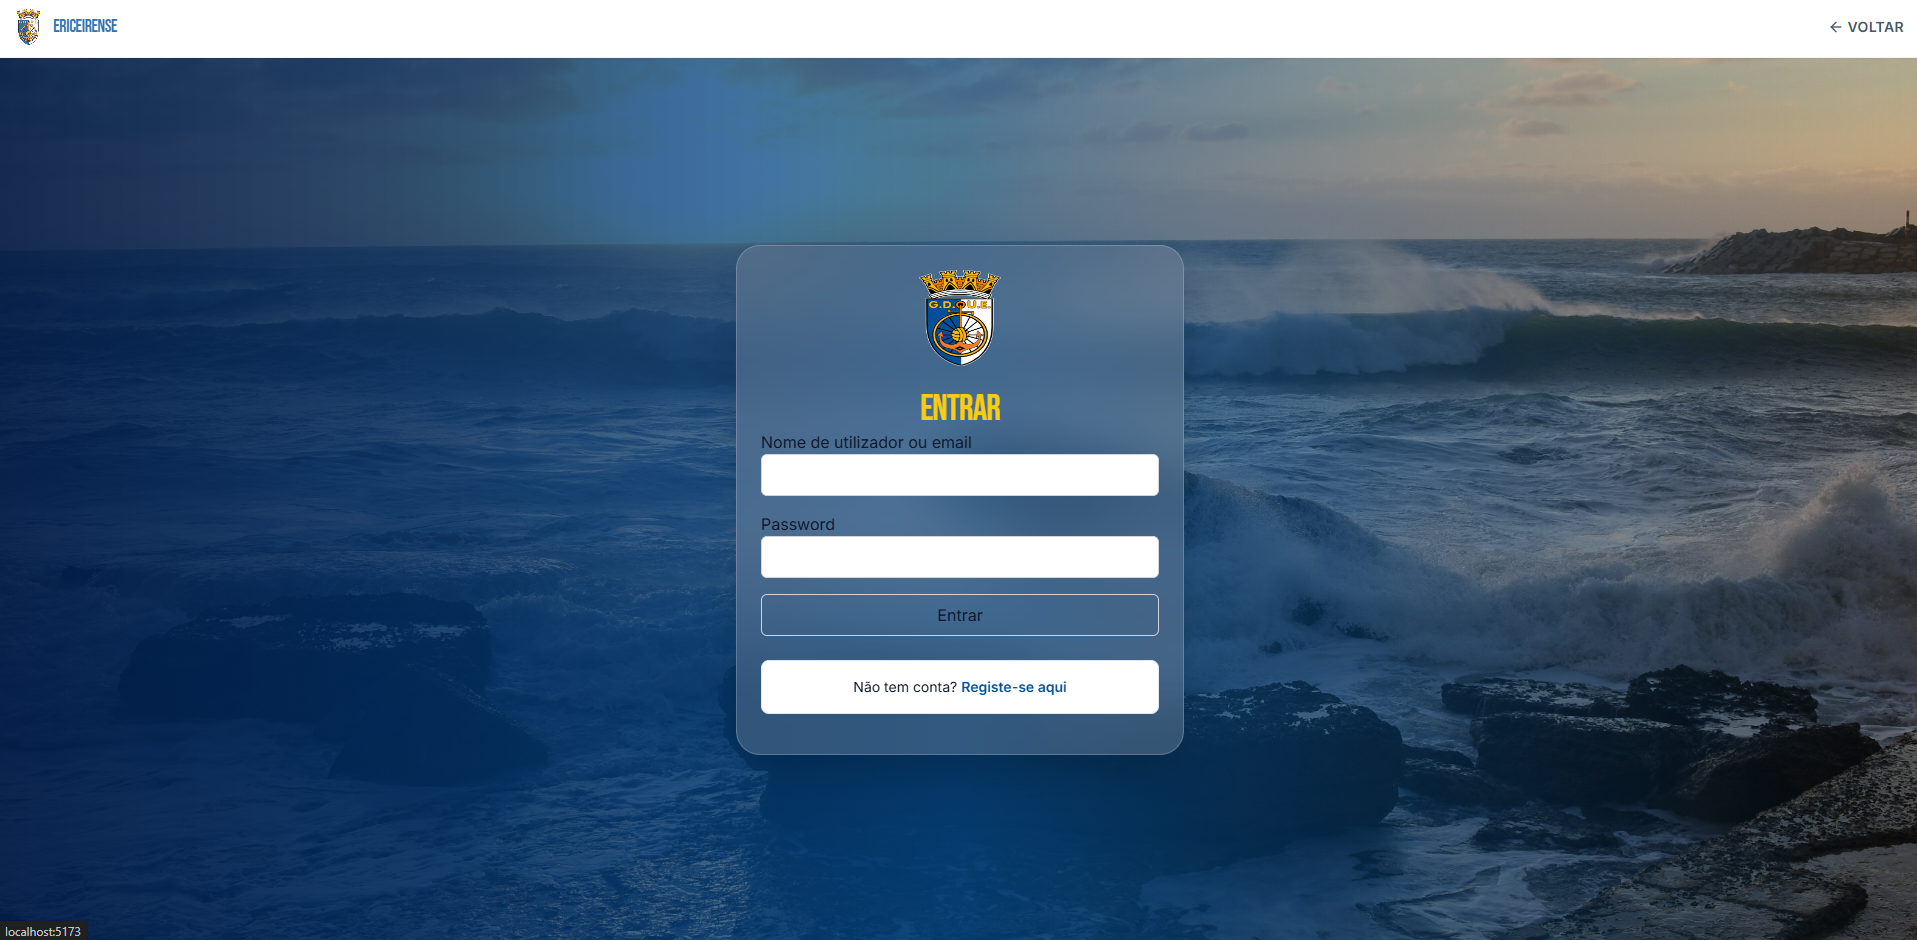
\includegraphics[width=\textwidth]{./figures/frontend-LoginPage.png}
    \caption{Página de autenticação}
    \label{fig:frontend-LoginPage}
\end{figure}

\subsection{Sócios}

A área de sócios permite criar, consultar, editar e gerir sócios do clube. No
lado público ou autenticado, o utilizador pode preencher o formulário de adesão,
introduzindo dados pessoais, contactos, morada, NIF, categoria e consentimentos.

Na área administrativa, os utilizadores com permissões podem consultar a lista
de sócios, aplicar filtros, aceder ao detalhe de cada sócio e executar ações de
gestão, como aprovação, rejeição, reativação, alteração de categoria ou edição
dos dados.

Esta funcionalidade inclui também a apresentação de informação financeira
associada ao sócio, nomeadamente quotas ou pagamentos pendentes, quando
aplicável. O acesso a recibos é feito através de ligações para os
\textit{endpoints} de pagamento disponibilizados pelo \textit{backend}.

\begin{figure}[H]
    \centering
    
    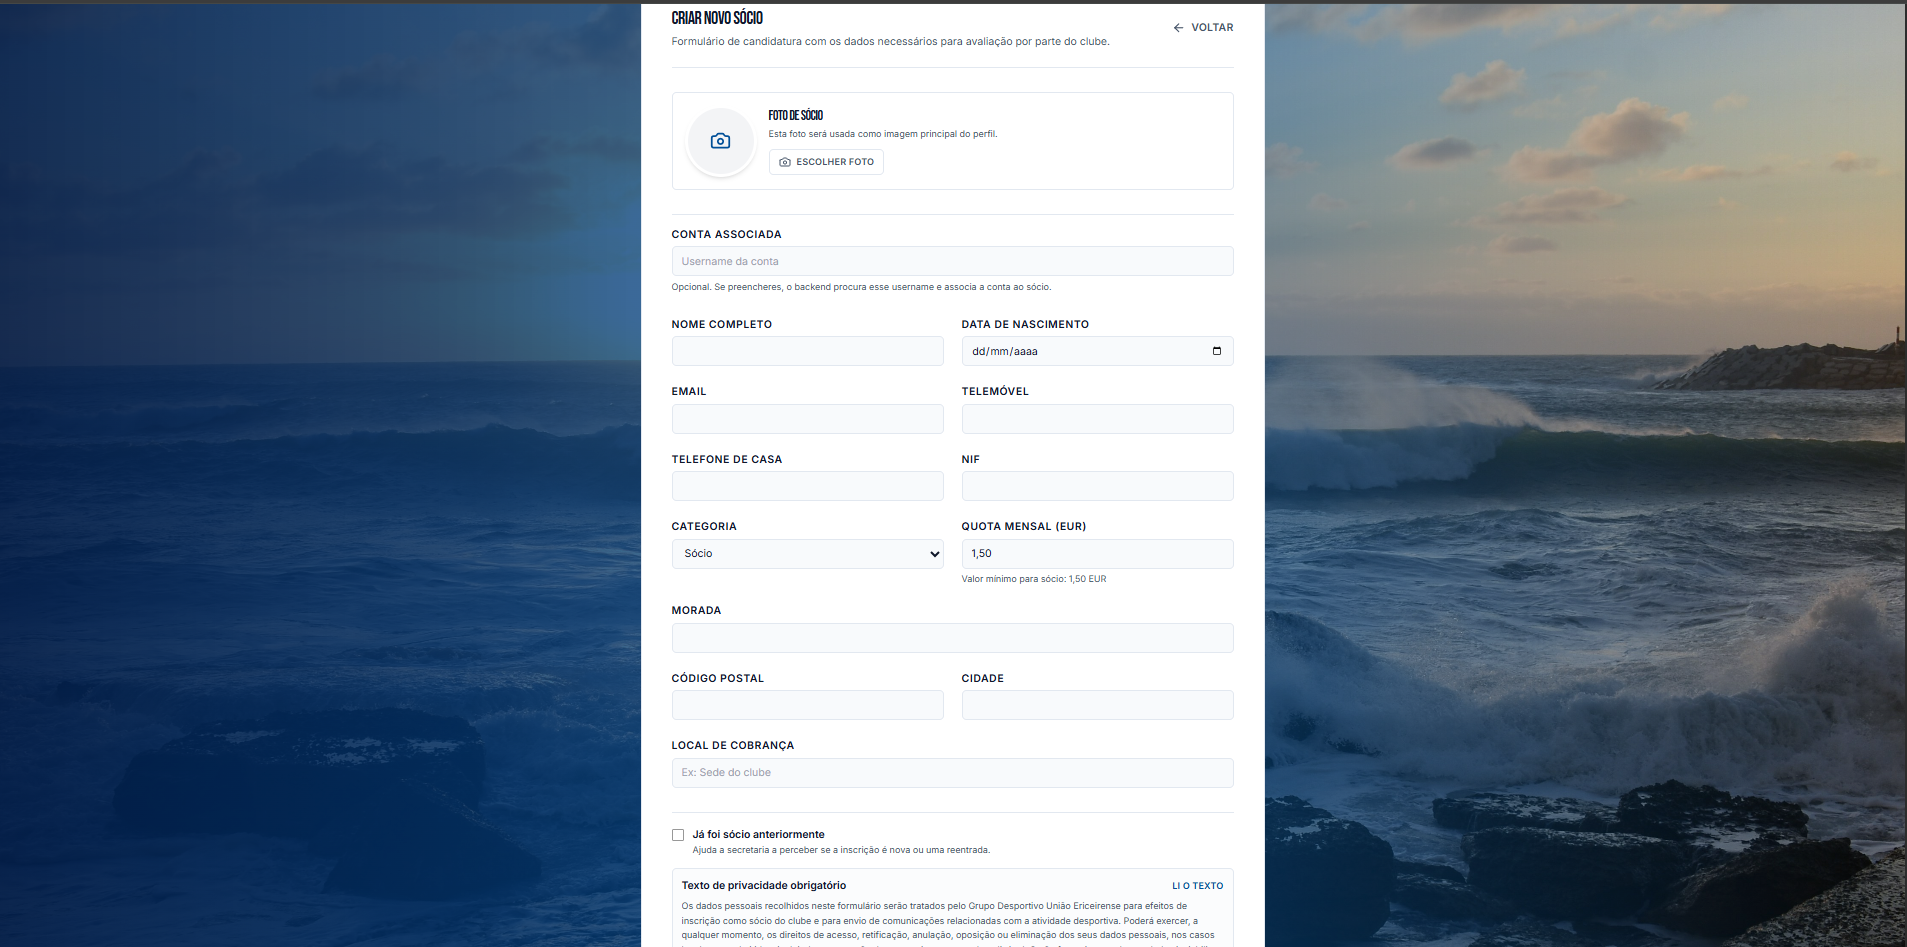
\includegraphics[width=\textwidth]{./figures/frontend-MemberFormPage.png}
    \caption{Formulário de adesão de sócio}
    \label{fig:frontend-MemberFormPage}
\end{figure}

\subsection{Atletas}

A funcionalidade de atletas suporta dois tipos principais de utilização. Por um
lado, permite a inscrição de novos atletas através de um formulário detalhado.
Este formulário recolhe dados pessoais, informação desportiva, dados escolares,
informação médica/administrativa e dados dos encarregados de educação.

Por outro lado, permite a consulta pública de atletas por escalão. Esta
consulta expõe apenas informação não sensível, como nome, número, posição,
nacionalidade, idade e escalão. Dados sensíveis, como documentos, contactos,
NIF, número de identificação ou dados de encarregados de educação, ficam
reservados à área administrativa.

Na área de gestão, os responsáveis podem consultar todos os atletas, incluindo
pendentes e rejeitados, editar dados administrativos, alterar o escalão,
aprovar ou rejeitar inscrições e ativar ou desativar atletas.

Existe ainda uma página de configuração de equipas, onde é possível gerir
grupos, escalões e tabelas de preços utilizadas nas opções de patrocínio
associadas a equipas.

\begin{figure}[H]
    \centering
    
    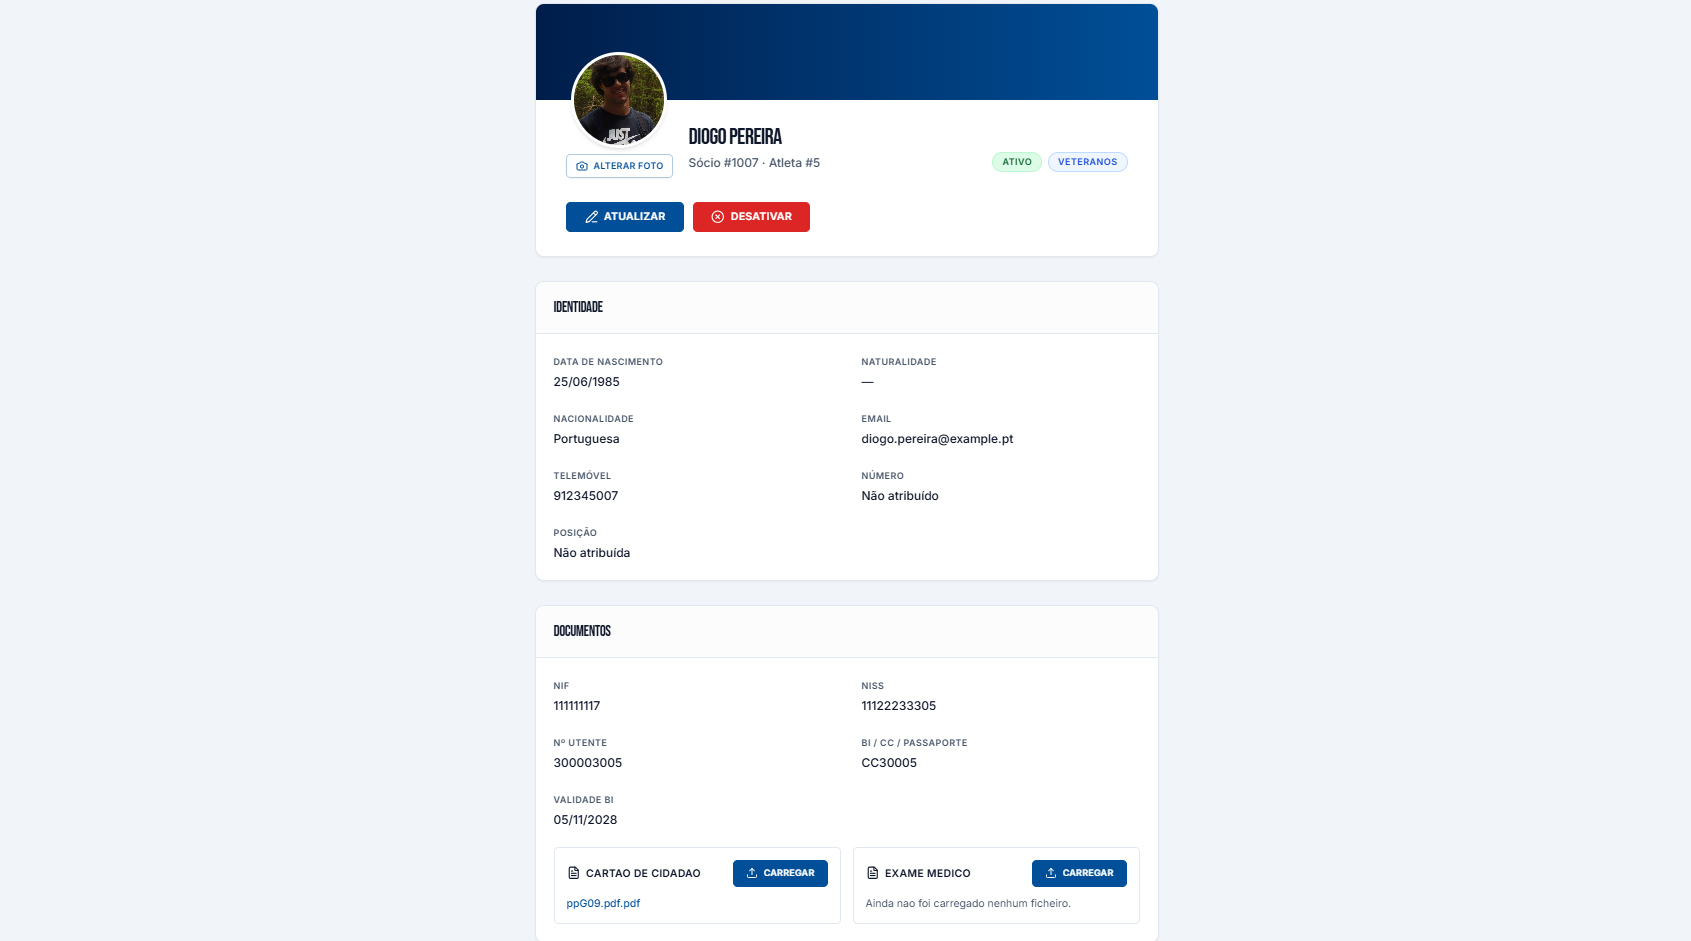
\includegraphics[width=\textwidth]{./figures/frontend-AthleteProfilePage.png}
    \caption{Página de perfil de atleta}
    \label{fig:frontend-AthleteProfilePage}
\end{figure}

\subsection{Patrocínios}

A área de patrocínios permite que um utilizador consulte informação sobre as
opções disponíveis e submeta um pedido de patrocínio. O sistema suporta
diferentes tipos de patrocínio, como publicidade em lona/outdoor, patrocínio de
equipas e apoio a outras modalidades ou iniciativas.

O \textit{frontend} apresenta os catálogos de opções disponíveis, calcula os
valores associados e permite a submissão do pedido. Para utilizadores
autenticados, existe também uma área de consulta dos seus próprios patrocínios,
onde podem acompanhar o estado de cada pedido e aceder aos detalhes ou recibos.

Na área administrativa, os responsáveis podem consultar todos os patrocínios,
aprovar pedidos, marcar pagamentos, cancelar contratos, gerir patrocinadores e
configurar os catálogos de opções. Esta configuração inclui opções de
publicidade, colocações em equipamentos, outras modalidades e regras de preços
por grupo ou escalão.

\begin{figure}[H]
    \centering
    
    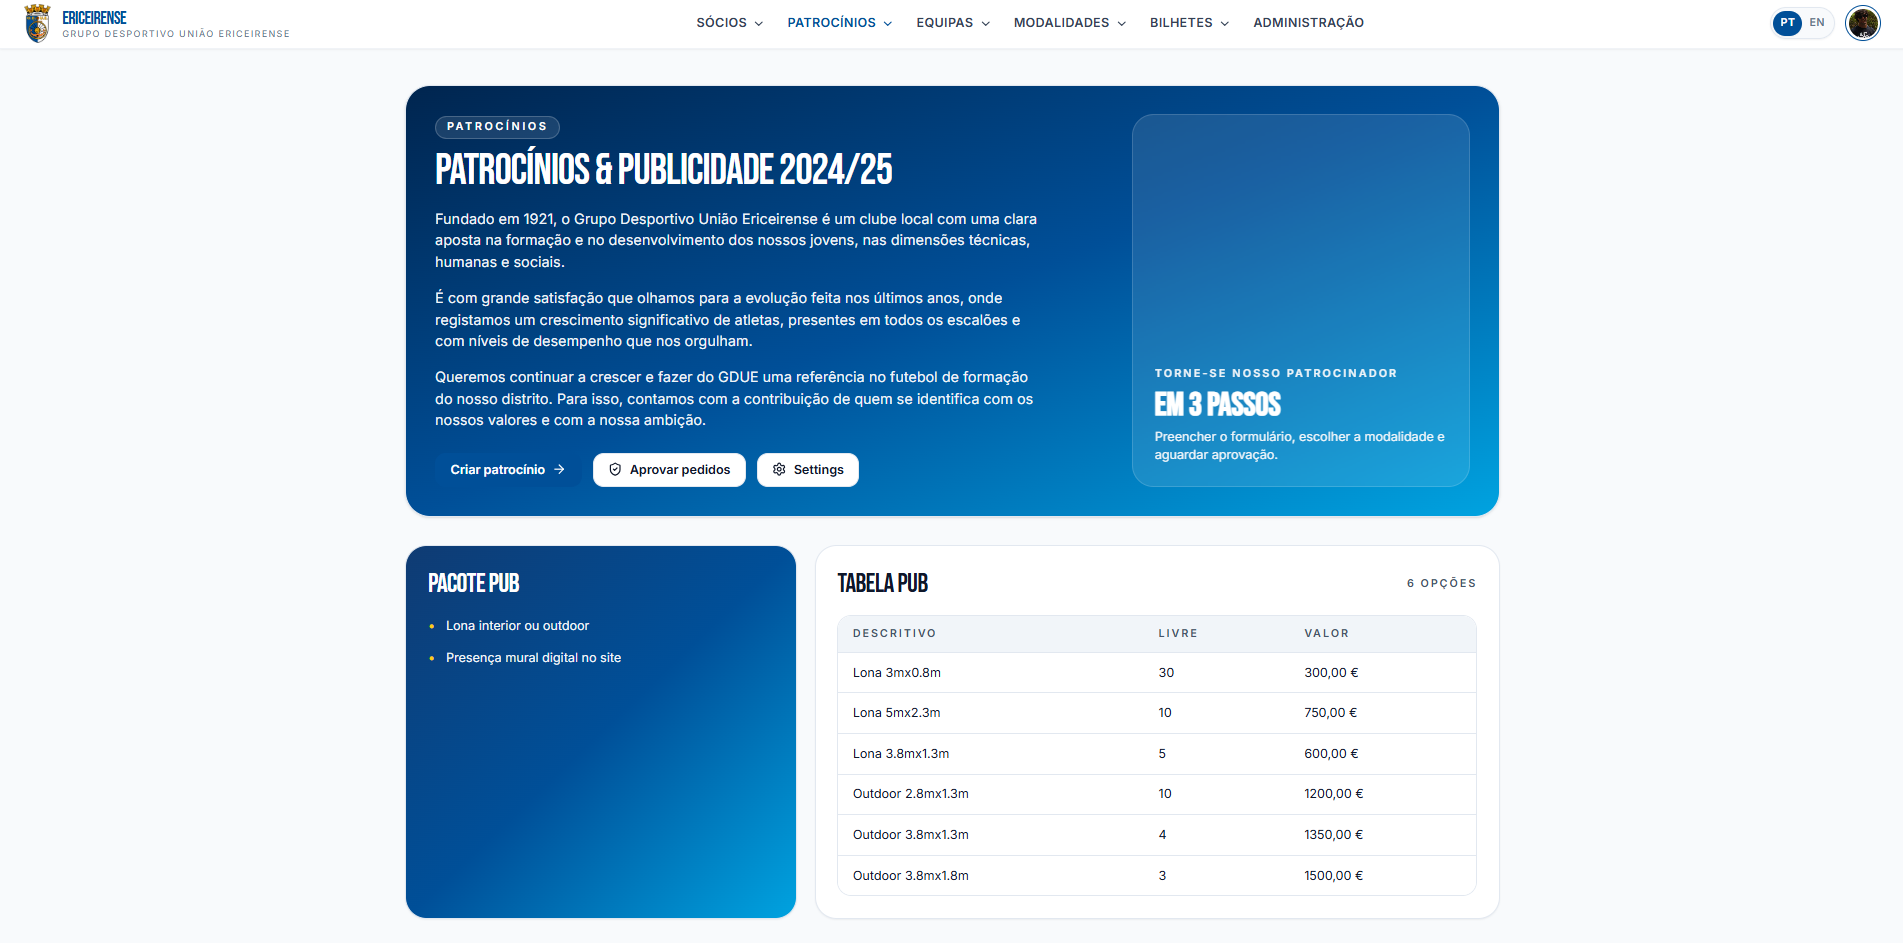
\includegraphics[width=\textwidth]{./figures/frontend-SponsorInfoPage.png}
    \caption{Página de Informação sobre Patrocínios}
    \label{fig:frontend-SponsorInfoPage}
\end{figure}

\subsection{Eventos e Bilheteira}

A funcionalidade de eventos permite criar e gerir jogos ou outros eventos do
clube. Na área administrativa, é possível criar eventos, definir descrição,
local, data, preços para público geral e sócios, e configurar setores com
lotação própria.

A área pública de bilheteira permite consultar eventos disponíveis e iniciar o
processo de compra de bilhetes. Durante este processo, o utilizador seleciona
os setores pretendidos e informa os dados necessários para a compra. Quando o
bilhete é de sócio, o sistema suporta a validação do número de sócio e da data
de nascimento, garantindo que o desconto é aplicado apenas a sócios válidos.

Após a criação da sessão de pagamento, o utilizador é redirecionado para o
serviço de pagamento. O \textit{frontend} possui ainda páginas específicas para
o resultado do pagamento, nomeadamente sucesso e cancelamento, acessíveis pelas
rotas \texttt{/payments/success} e \texttt{/payments/cancel}.

\subsection{Utilizadores e Perfil}

A área de utilizadores permite ao utilizador autenticado consultar o seu perfil
e as entidades a si associadas, como sócio, atleta ou patrocinadores. Na área
administrativa, os responsáveis podem consultar a lista de utilizadores, aceder
ao detalhe de cada um, alterar o papel atribuído e associar um sócio ativo.

Esta funcionalidade é importante para ligar a autenticação às entidades do
domínio do clube. Um utilizador pode ter permissões diferentes consoante o seu
papel, mas também pode estar associado a um sócio ou patrocinador, o que
influencia as ações que pode realizar.

\subsection{Ficheiros}

A aplicação inclui uma funcionalidade dedicada à gestão de ficheiros, utilizada
por várias áreas do sistema. Esta funcionalidade permite listar, carregar,
consultar e remover ficheiros associados a entidades como utilizadores, sócios
ou atletas.

No \textit{frontend}, esta gestão é encapsulada em componentes e funções de API
próprias. Os ficheiros são enviados através de pedidos
\texttt{multipart/form-data}, adequados ao envio de conteúdo binário. Para
visualização ou acesso aos ficheiros, a aplicação constrói ligações para os
\textit{endpoints} do \textit{backend}, como o conteúdo de um ficheiro ou a
fotografia pública de um atleta.

A utilização desta funcionalidade permite manter a gestão documental integrada
na aplicação, sem misturar o conteúdo binário com os dados estruturados
apresentados nos formulários.

\subsection{Administração}

A área de administração funciona como o \textit{backoffice} da aplicação. O seu
acesso está reservado a utilizadores com os papéis \texttt{ADMIN} ou
\texttt{SECRETARIA}. Esta área reúne as ferramentas necessárias para gerir o
funcionamento do clube.

O painel inicial apresenta estatísticas gerais, permitindo obter uma visão
rápida sobre o estado da organização, como número de sócios, atletas,
patrocínios ou pedidos pendentes. A partir deste painel, os responsáveis podem
navegar para as diferentes áreas de gestão: sócios, atletas, utilizadores,
patrocínios, eventos e configurações.

\begin{figure}[H]
    \centering
    
    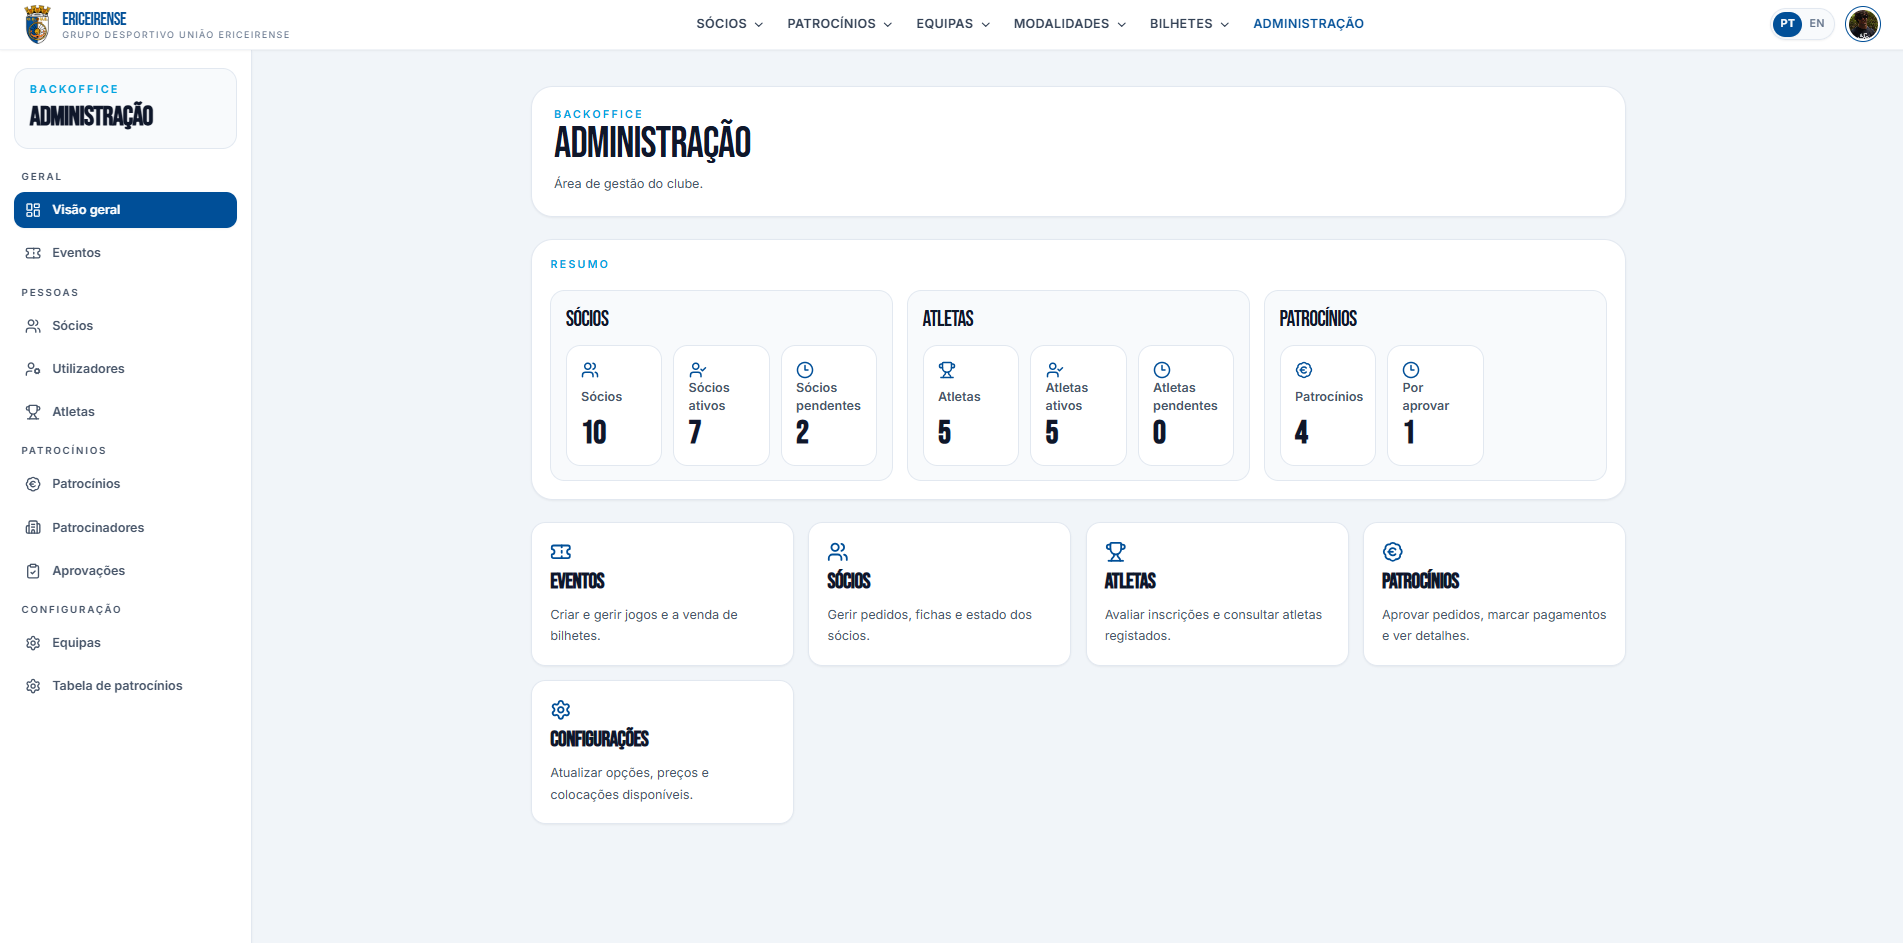
\includegraphics[width=\textwidth]{./figures/frontend-AdminPage.png}
    \caption{Página Inicial do BackOffice}
    \label{fig:frontend-AdminPage}
\end{figure}

\section{Formulários e Validação}

Uma parte significativa da aplicação é composta por formulários, uma vez que os
principais processos do clube envolvem recolha de dados: adesão de sócios,
inscrição de atletas, criação de patrocínios, edição de utilizadores e criação
de eventos.

Os formulários são estruturados em componentes específicos, como
\texttt{MemberForm} e \texttt{AthleteForm}, e utilizam tipos TypeScript para
representar os dados esperados. Para facilitar a inicialização e transformação
dos valores dos formulários, existem ficheiros utilitários como
\texttt{formValues.ts}, que concentram valores por omissão e conversões
necessárias antes do envio para a API.

A validação é feita em dois níveis. No \textit{frontend}, são aplicadas
validações imediatas que melhoram a experiência do utilizador, como campos
obrigatórios, formatos de datas, valores numéricos e conversões monetárias. No
\textit{backend}, as regras de negócio são novamente validadas, garantindo que
a integridade dos dados não depende apenas da interface.

Esta dupla validação é importante porque o \textit{frontend} melhora a
usabilidade, mas o \textit{backend} continua a ser a fonte de verdade das
regras da aplicação.

\section{Tipos e Segurança em Tempo de Desenvolvimento}

A utilização de TypeScript permite declarar tipos para os dados manipulados
pela aplicação. Cada funcionalidade define os seus próprios tipos, como
\texttt{Member}, \texttt{Athlete}, \texttt{Sponsorship}, \texttt{Event} ou
tipos auxiliares de formulários.

Esta tipagem contribui para reduzir erros durante o desenvolvimento. Por
exemplo, se uma função espera um identificador numérico ou um determinado
campo obrigatório, o compilador consegue assinalar usos incorretos antes da
execução da aplicação. Isto torna o código mais previsível e facilita a
refatoração.

A tipagem é especialmente útil na comunicação com a API, uma vez que as
respostas do \textit{backend} são convertidas para estruturas conhecidas no
\textit{frontend}. Embora esta validação não substitua a validação no servidor,
ajuda a manter consistência entre as duas camadas.

\section{Tratamento de Estados da Interface}

As operações assíncronas, como carregamento de listas, submissão de formulários
ou atualização de dados, exigem a representação de diferentes estados na
interface. A aplicação distingue estados como carregamento, sucesso, erro e
ausência de dados.

Esta distinção permite fornecer uma experiência mais clara ao utilizador. Por
exemplo, durante o carregamento de uma lista, a interface pode apresentar uma
mensagem ou indicador de espera; em caso de erro, pode mostrar uma mensagem
descritiva; e após uma operação bem-sucedida, pode redirecionar o utilizador ou
apresentar confirmação.

A existência de funções e \textit{hooks} auxiliares para este tratamento evita
que cada componente implemente de forma diferente a mesma lógica de estado.

\section{Estilo Visual e Responsividade}

O estilo visual da aplicação combina CSS próprio com Tailwind CSS. As folhas de
estilo específicas de cada funcionalidade permitem controlar detalhes visuais
de páginas complexas, como formulários, painéis de administração, cartões,
listas e tabelas. O Tailwind CSS é utilizado como base utilitária e para
definir um tema coerente.

A aplicação procura refletir a identidade visual do clube, recorrendo a imagens
e elementos gráficos presentes na pasta pública, como o logótipo e imagens de
fundo. Estes elementos ajudam a aproximar a interface da identidade institucional
do GDUE.

A responsividade é uma preocupação importante, uma vez que a aplicação pode ser
utilizada tanto em computadores como em dispositivos móveis. A interface é
organizada para se adaptar a diferentes larguras de ecrã, especialmente nas
áreas públicas, como a página inicial, consulta de atletas, inscrição e compra
de bilhetes. Nas áreas administrativas, onde existe maior densidade de
informação, a prioridade é manter a leitura clara e a navegação eficiente.

\section{Internacionalização}

Uma das funcionalidades relevantes do \textit{frontend} é o suporte a múltiplos
idiomas, através de um módulo de internacionalização (i18n). Esta funcionalidade
foi considerada importante no contexto do clube, uma vez que a Ericeira conta
atualmente com uma comunidade internacional significativa: o clube integra
cerca de 20 nacionalidades diferentes, na sua maioria sem o português como
língua oficial. Neste contexto, o suporte ao idioma inglês tornou-se um
requisito mínimo para garantir o acesso desta comunidade às funcionalidades da
aplicação.

A internacionalização foi implementada com recurso à biblioteca
i18next~\cite{i18next} e à sua integração com o React. A aplicação suporta dois
idiomas, português e inglês, mantidos em paridade. As traduções de cada idioma
estão organizadas num ficheiro próprio, estruturado em secções correspondentes
às diferentes áreas da aplicação.

A seleção do idioma é automática na primeira utilização: a aplicação deteta o
idioma preferido do utilizador e, na ausência de informação, assume o português
por omissão. A escolha do utilizador é memorizada para utilizações seguintes. É
ainda possível alternar manualmente entre os idiomas disponíveis através de um
seletor presente no cabeçalho da aplicação. Os componentes consomem as
traduções através de uma função dedicada, que permite também a inserção de
valores dinâmicos no texto traduzido.
